\section[Integral geometry. Or ``How long is a piece of string?'']{Integral geometry\\ {\large Or ``How long is a piece of string?''}}
\label{sec:integral-geometry}

\subsection{Motivation}

Geometry has been a recurring theme in physical theories, appealing because of its intuitive nature.
There are many ways that geometric ideas can be incorporated, but our focus will be on expansions of thermodynamic quantities in terms of \emph{sizes}.
The usefulness of this particular focus is directly connected to the familiar concept of \emph{extensivity} in statistical mechanics, which we will use to guide the following discussion.
Thermodynamic potentials must be extensive to remain well-defined in the thermodynamic limit.
%Defining an extensive quantity as one that scales proportionally to system size, the first meaning of size that comes to mind is probably the volume.
So by focusing on quantities which are extensive we ensure a thermodynamic description which is consistent in this limit.

%The first notion of size that likely comes to mind is the volume, though we will generalise to all reasonable notions of size.
%The simplest example we can give is from statistical mechanics: an \emph{extensive variable} is one that scales proportionally to the system volume.
%For a finite system $K \subset \mathbb{R}^d$ %the volume is expressed
%% \begin{equation}
%%   V[K] = \int_K d\vec{r}.
%% \end{equation}
%Then,
As an example, extensive quantities includes the \emph{entropy} of a large system which can be expressed in terms of system volume as
\begin{equation*}
  S = s V
\end{equation*}
where $s$ would be an entropy density which is \emph{intensive}, meaning it does not change with system volume.
Another example is the surface energy of a macroscopic surface, which can be written
\begin{equation*}
  E = \gamma A
\end{equation*}
where $\gamma$ is the surface tension and $A$ is the surface area.
More refined notions of extensivity invoke homogeneity of arguments \cite{Chandler1987}
\begin{equation}\label{eq:extensive-homogeneity}
  \phi(\cdot).
\end{equation}
We will explore what other reasonable notions of `size' there may be, in the hope that we arrive at ideas that prove useful in developing new theories.
We will begin by listing some examples of other possible notions of size.

\hl{We now introduce curvature, ideas from differential geometry.}
A surface is a two-dimensional manifold so its local shape is described by two basis vectors.
Supposing the surface is parameterised by coordinates $(x_1, x_2)$, then the basis vectors at a point on the surface $\vec{r}$ are
\begin{equation}
  \vec{e}_\alpha := \frac{\partial \vec{r}}{\partial x_\alpha}
  \qquad \alpha \in \{1, 2\}.
\end{equation}
Then, the shape of the surface is characterised by changes in the basis vectors leading to the curvature tensor
\begin{equation}
  \kappa_{\alpha \beta} := \frac{\partial \vec{e}_\beta}{\partial x_\alpha}
  \qquad \alpha, \beta \in \{1, 2\}.
\end{equation}
The values of the curvature tensor will depend on the choice of coordinate system $(x_1, x_2)$, so it is usual to consider the \emph{curvature invariants}, i.e.\ the trace and determinant%
\marginfootnote{This argument is readily generalised to $(d-1)$-dimensional surfaces in $\mathbb{R}^d$, where we would find $d-1$ invariants of the curvature tensor.},
leading to the the \emph{mean} and \emph{Gaussian curvatures}
\begin{subequations}
  \begin{align}
    H &:= \frac{\Tr{\kappa}}{2}, \\
    G &:= \det{\kappa}.
  \end{align}
\end{subequations}
As an example of how curvature can be a useful concept in statistical mechanics, we put forward the Young-Laplace equation which writes the pressure difference between two fluids as
\begin{equation*}
  \Delta p = 2 \gamma H,
\end{equation*}
with applications to e.g.\ phase coexistence \cite{YoungPTRSL1805,Laplace1805} or frost damage to porous solids \cite{EverettTFS1961}.
Extensive curvature measures are obtained by integrating the curvature invariants over the surface, leading to the integrated mean and Gaussian curvatures $C$ and $X$.

Together, the extensive geometric measures we have introduced so far can be written as%
\marginfootnote{We use the usual physicist abuse of notation where $V$ refers to both a region in space $V \subset \mathbb{R}^d$, and also the physical volume of this space.}
\begin{subequations}\label{eq:intrinsic-volumes-surface-integrals}
  \begin{align}
    V
    &=
    \int_V \, d\vec{r},
    \\
    A
    &=
    \int_{\partial V} \, d\vec{r},
    \\
    C
    &=
    \int_{\partial V} H(\vec{r}) \, d\vec{r},
    \\
    X
    &=
    \int_{\partial V} G(\vec{r}) \, d\vec{r}.
  \end{align}
\end{subequations}
The latter three quantities are \emph{expressed} here as the surface integrals, but we shall see that they are really size measures on the volume $V$.
It turns out that these are the \emph{only} reasonable notions of size in three-dimensions, a central finding in the field of \emph{integral geometry}.
%is a powerful tool for incorporating intuitive, flexible ideas into theories.
%For this reason geometric approaches are common in statistical mechanics such as the Young-Laplace equation, which corrects Asakura-Ozawa

Other examples of theories which incorporate notions of size include the Asakura-Ozawa, which describes depletion forces using exclusion volumes, and more generally any free volume theory which expresses an energy in terms of a volume in space.
We introduce the field of \emph{integral geometry} which generalises the underlying geometric principles of these theories into a unified framework for characterising size.
\todo{Repetition}
%% We could argue that fundamentally these theories are based on measuring physical sizes.
%% Integral geometry offers a mathematically rigorous formalism for describing sizes, so presents a possible starting point for free volume theories.
This mathematical formalism provides elegant and unified description of sizes, and was crucial in the development of modern theories of hard spheres including the main ideas underlying chapters \ref{chapter:morphometric-framework}, \ref{chapter:morphometric-applications} and \ref{chapter:resummation}.
%Ideas from this branch of mathematics were crucial to the development of fundamental measure theory (section \ref{sec:fmt}), so it makes sense to place this before the section on liquid state theory.
As integral geometry is generally unfamiliar to people with a background in physics, we will place emphasis on the concepts and intuition rather than rigour.

\subsection{What do we even mean by size?}

We will now make our notion of `size' more precise.
At the same time, we must precisely specify which objects this definition applies to.

First we define our objects: sets in Euclidean space.
We will see that the only reasonable notion of size is a \emph{continuous} rigid-motion invariant valuation.

We could completely describe the size of simple objects by completely defining their geometry, e.g.\ the dimensions of a box.
This is of course sufficient, however it is not very useful.
However, this may not be straightforward for more complex objects, and by abstracting the problem somewhat we can obtain useful theorems etc.
%% We now give a brief justification of the above \emph{ansatzes}, in particular why there are only four terms in the expansion.
%% Radius is the only natural parameter for a sphere, however for more general geometries there might be arbitrarily many parameters so one may wonder if they should be included in a general geometric expansion.

So we have to generalise what we mean by size, simultaneously we will have to carefully specify what objects we wish to measure.
We might naively select all subsets of $\mathbb{R}^d$, however this leads to pathological problems; the Banach-Tarski paradox ensues.
We need to be precise with what kind of geometries we consider: a definition too broad may not allow meaningful size measures, while a narrow definition may cease to be useful.

We consider polyconvex sets%
\marginfootnote{The set of polyconvex objects is also sometimes called the \emph{convex ring}.}.
Avoid pathological sets: Banach-Tarski paradox allows one to break a sphere apart and recompose it as two identical spheres.
We want a well-defined volume, so need to avoid sets which allow this.
\marginfootnote{Have to be formed by countable union of convex objects.
Covers most physically realistic geometries.}

%% The first intuitive notion for a size: the size of nothing is zero, i.e.:
%% where $\emptyset$ is the empty set.
%% A box: take the largest length, but then the `size' is not increased by modifying its smallest dimensions.
%% Ideally, we want a size measure that increases monotonically as we add additional material. This leads to additivity:
%% \begin{equation}
%%   \phi(A \cup B) = \phi(A) + \phi(B) - \phi(A \cap B)
%% \end{equation}
%% Connection with entropy, leads to homogeneity in arguments which is the building block for extensivity of a thermodynamic potential.
%% This provides a geometrically precise foundation for thermodynamic potentials.

We put forward the following qualities of the measures $V, A, C$ and $X$ which make them intuitive notions of size:
\begin{enumerate}
\item They are invariant with respect to translations and rotations, so that an object's size is independent of the observer.
\item They increase additively, i.e.\ they transform under combination of subsystems via the inclusion/exclusion relation e.g.\ for two objects $K_1$ and $K_2$
  \begin{equation}\label{eq:additivity}
    V[K_1 \cup K_2] = V[K_1] + V[K_2] - V[K_1 \cap K_2],
  \end{equation}
  and similar expressions for $A$, $C$, and $X$.
  As corollaries, this property contains the expectation that the size of nothing is zero, i.e.\ $V[\emptyset] = 0$ and the homogeneity property of extensive variables \eqref{eq:extensive-homogeneity}.
\item They are continuous%
  \marginfootnote{Specifically, in integral geometry this continuity property is with respect to the \emph{Hausdorff metric}.
    Details on this can be found in standard texts, e.g.\ Refs.\ \cite{Santalo2004,Klain1997}.}.
  Loosely speaking, this means that the size measures converge as the object is approximated by increasingly finely meshed polyhedra excluding e.g.\ fractal geometries.
  As a simple intuitive example, the measurement of a length will converge continuously to some number as one uses rulers with progressively finer distance markings.
\end{enumerate}
The final property specifically excludes geometries for which we do not expect there to be any reasonable measurement of size.

Compactness:
\begin{itemize}
\item \emph{Bounded}: the body must be finite in scope, as no meaningful size can be defined for a body spanning an infinite region of space.
\item \emph{Closed}: the body contains its boundary.
  This is an important property which we will see by example in discussing the Gauss-Bonnet theorem below.
\end{itemize}
The empty set $\emptyset$ is a compact body, albeit a special case with zero size.
Compact convex set $K \in \mathcal{K}$ notation.

\subsection{Aside: the Euler characteristic}

Aim of this section is to provide intuition over Euler characteristic.

Repeat arguments in figures and you obtain the general rule that dividing an $n$-sphere gives two $n-1$-dimensional convex objects and a $n-1$ sphere dividor.
This gives us the rule for the Euler characteristic.
Euler characteristic describes the topology.

\begin{itemize}
\item Multiple disjoint convex objects: increase
\item Holes lower Euler characteristic
\item Cavities increase
\end{itemize}

For $d=3$ we have the important Gauss-Bonnet theorem.

The only convex object in 1d is a line segment.

%% \begin{SCfigure}[H]
%%   \missingfigure[figwidth=0.5\linewidth]{$\partial B$}%
%%   \missingfigure[figwidth=0.5\linewidth]{$\partial B$}
%%   \caption{Effect of holes: divide 2d circle in two (2 rods + 2 points).}
%% \end{SCfigure}

%% \begin{SCfigure}[H]
%%   \missingfigure[figwidth=0.5\linewidth]{$\partial B$}%
%%   \missingfigure[figwidth=0.5\linewidth]{$\partial B$}
%%   \caption{Effect of cavities: divide 3d sphere in two (2 discs + circle).}
%% \end{SCfigure}

\begin{tcolorbox}[title=A note on nomenclature]
  The terms `sphere' and `ball' are used interchangeably in physics (and colloquially), however in geometry these refer to different things; `ball' refers to the solid object whereas `sphere' refers to its boundary, i.e.\
  \begin{equation*}
    S^{d-1} = \partial B^d,
  \end{equation*}
  As a surface manifold, the $(d-1)$-dimensionality of the sphere is reduced by one from its original space.
  So strictly speaking, when we speak of hard spheres in physics we really mean hard balls%
  \marginfootnote{Strictly speaking the interactions between hollow spheres and solid balls would be identical, so it is possible to still speak of hard spheres.
    However, typically we always exclude geometries where spheres contain each another so hard balls better capture the interactions of interest.
    Moreover, colloidal hard spheres are solid.}
  in the geometric sense.
\end{tcolorbox}

Should explain intrinsic volumes earlier perhaps.
Euler characteristic of a boundary depends on dimension:
\begin{align}
  \chi(K^d) &= 1 \\
  \chi(\partial K^d) &= 1 + (-1)^d
\end{align}
Disjoint union: sum them (by inclusion-exclusion principle).

Euler characteristic is the simplest size measure: why is this a size measure?
\marginfootnote{As an illustration of why this is a size measure, I like to imagine that the \emph{size} of a pirate's treasure is the \emph{number} of gold coins in their possession, which is the Euler characteristic of their hoard.}

\begin{theorem}{Gauss-Bonnet theorem}
  Using the additivity property we can decompose the Euler characteristic into a surface and interior term
  \begin{equation*}
    \chi(\partial K) + \chi( \interior(K) ) = \chi(K) = 1
  \end{equation*}
  using the fact that the Euler characteristic of a compact body is unity.
\end{theorem}

The main point of this theorem is that it establishes an equivalence between two seemingly distinct measures of size (? could be equivalence between surface measure and volume one): Gaussian curvature and Euler characteristic.
For a spherical solute these reduce to the values given in \eqref{eq:spt-ansatz}, so this represents a proper generalisation of SPT for more general geometries.

\subsection{Generalisation: intrinsic volumes}

To obtain results for all physical dimensions $d \le 3$ it is convenient to generalise the morphometric \emph{ansatz} \eqref{eq:morphometric-approach} to arbitrary $d$ and substitute $d \in \{1, 2, 3\}$ at the end of our derivation.
To that end it is convenient to introduce generalisations of the geometric parameters $\{V,A,C,X\}$: the \emph{intrinsic volumes} $\{V_d, V_{d-1}, \cdots, V_0\}$.
To introduce the intuition behind these generalised volumes we start from the observation that the quantities $\{V,A,C,X\}$ can be imagined as size descriptors for projections onto $k$-dimensional subspaces in $\mathbb{R}^3$; for a compact body $K \subset \mathbb{R}^3$ we have:
\begin{enumerate}
\item $V(K)$ is trivially the volume of the intersection of $K$ with the 3-dimensional subspace i.e.\ all of Euclidean space.
\item $A(K)$ can be thought of as the typical size of two-dimensional images formed by projections onto planes.
\item $C(K)$ is related to the projections onto one-dimensional subspaces i.e.\ lines.
  This curvature measure is normally thought of as a surface property, but this definition suggests an equivalence (up to a different normalisation) with the \emph{mean width} $L(K)$ of the body.
\item $X(K)$ is obtained from projections onto a single point; this surface measure is thus equivalent to the Euler characteristic $\chi(K)$.
  This connection results in the celebrated Gauss-Bonnet theorem of differential geometry, which we would write
  \begin{equation*}
    X(K) = 2\pi \chi(K)
  \end{equation*}
  in our notation.
\end{enumerate}

Generalising the above intuition to $d$-dimensions, we see that in general we can imagine $d+1$ projections and so expect $d+1$ corresponding volumes.
We define the $k$th intrisic volume as the average size of the projections onto $k$-dimensional linear subspaces of $\mathbb{R}^d$, i.e.\
%Denoting the space of all $k$ dimensional linear subspaces in $\mathbb{R}^d$ as $\mathrm{Graff}(d,k)$ (the affine Grassmanian), the intrinsic volume is obtained by
\begin{equation}\label{eq:intrinsic-volumes}
  V_k(K)
  =
  C_{k,d-k}
  \int \chi(K \cap E_{d-k}) \, d\mu(E_{d-k})
\end{equation}
where the integral is taken over all affine transformations of the plane $E_k$ in $\mathbb{R}^d$ and the flag coefficient is
\begin{equation}\label{eq:flag-coefficients}
  C_{k,d-k}
  :=
  \frac{d!}{k! (d-k)!} \frac{\omega_d}{\omega_k \omega_{d-k}},
\end{equation}
where the volume of the $d$-dimensional unit ball is
\begin{equation}
  \omega_d := V_d(B^d) = \frac{\pi^{d/2}}{\Gamma(\frac{d}{2} + 1)}.
\end{equation}
The flag coefficients $C_{k,d-k}$ have a similar structure to binomial coefficients, and play a similar \emph{combinatorial} role for combining subspaces (section \ref{sec:kinematic-formula}).
By convention, the normalisation of the measure $d\mu(E_{d-k})$ in \eqref{eq:intrinsic-volumes} is chosen to give the intrinsic volumes for the $d$-dimensional unit ball $B^d$ as
\begin{equation}\label{eq:intrinsic-volume-ball}
  V_k (B^d)
  =
  {d \choose k} \frac{\omega_d}{\omega_{d-k}}.
\end{equation}
%The intrinsic volumes thus only depend on the dimensionality of the body, not the embedding space.
A set of common geometrical quantities and their reduction to the intrinsic volumes in physical dimensions $d \le 3$ is given in Table~\ref{table:geometric-quantities}.
Finally, with the intrinsic volumes the generalisation of the morphometric apparoach \eqref{eq:morphometric-approach} for a solute $K$ in $d$-dimensions reads
\begin{equation}\label{eq:morphometric-approach-d}
  \Delta \Omega(K)
  =
  \sum_{k=0}^d a_k V_k(K).
\end{equation}

\begin{SCtable}
  \begin{minipage}[b]{\linewidth}
    \centering
    \begin{tabular}{ccccc}
      \toprule
      $k$ & $\omega_k$ & $V_k(B_1)$ & $V_k(B_2)$ & $V_k(B_3)$ \\
      \midrule
      0 & 1 & 1 & 1 & 1 \\
      1 & 2 & 2 & ? & 4 \\
      2 & $\pi$ && $\pi$ & $2\pi$ \\
      3 & $\frac{4\pi}{3}$ &&& $\frac{4\pi}{3}$ \\
      \bottomrule
    \end{tabular}
  \end{minipage}
  \caption{Intrinsic volumes of the unit ball in physical dimensions $d \le 3$.}
\end{SCtable}

\begin{theorem}{Hadwiger's characterisation theorem}
  Together the functionals $\{\mu_k\}_{k=0}^d$ form a basis for the vector space of all continuous rigid-motion invariant valuations on polyconvex sets in $\mathbb{R}^d$.
I.e. a continuous rigid-motion invariant valuation can be written
\begin{equation}
  \mu(A) = \sum_{i=0}^d c_i \mu_i(A)
\end{equation}
where $c_i$ are some coefficients independent of $A$.
\end{theorem}

The basis of the morphometric approach is that the functionals $\{V,A,C,X\}$ are normalisations of the so-called \emph{intrinsic volumes}.
These play a central role in integral geometry as the \emph{only} physically meaningful size measures in the sense that they:
\begin{enumerate}
\item Are invariant with respect to translations and rotations.
\item Increase additively, i.e.\ they transform under combination of subsystems via the inclusion/exclusion relation e.g.\
  \begin{equation*}\label{eq:additivity}
    V[A \cup B] = V[A] + V[B] - V[A \cap B],
  \end{equation*}
  and similar expressions for $A$, $C$, and $X$.
\item Are continuous (specifically with respect to the Hausdorff metric).
  Loosely speaking, this means that the size measures converge as the object is approximated by increasingly finely meshed polyhedra excluding e.g.\ fractal geometries.
  As a simple intuitive example, the measurement of a length will converge continuously to some number as one uses rulers with progressively finer distance markings.
\end{enumerate}
More details on properties of intrinsic volumes can be found in standard texts, e.g.\ Refs.\ \cite{Santalo2004,Klain1997}.
%\cite{Santalo2004,SchneiderACIG1984,Schneider2008,Klain1997}.

The central assertion of the morphometric approach is that the insertion cost $\Delta \Omega$ \emph{exactly} possesses the properties above, providing the connection between geometry and thermodynamics \cite{KonigPRL2004}.
A classic theorem of integral geometry due to Hadwiger \cite{Hadwiger1957} states that the intrinsic volumes are the \emph{only} class of functionals with the properties listed above; a corollary of this is that they form a linear vector space for any functional possessing these properties.
The morphometric form \eqref{eq:morph-ansatz} then follows.
In addition to providing a more general \emph{ansatz} than SPT, this approach lays out its underlying assumptions explicitly eschewing the ad-hoc way in which the original SPT \emph{ansatz} \eqref{eq:spt-ansatz} was obtained.

The morphometric approach is certainly an approximation, as the insertion cost will not rigorously possess the three properties above in reality.
Notably, in SPT $\Delta\Omega$ is known to contain singularities in its high order derivatives with solute radius \cite{ReissJCP1959}; these non-analytic terms result from violations of the additivity assumption.
Nevertheless, the approximation is accurate in hard spheres \cite{OettelEL2009,AshtonPRE2011,LairdPRE2012,BlokhuisPRE2013,UrrutiaPRE2014,Hansen-GoosJCP2014} so these violations should be small.

\begin{SCtable}
  \begin{minipage}[b]{\linewidth}
    \centering
    \begin{tabular}{ccc}
      \toprule
      \multicolumn{2}{c}{Geometric quantity} \\
      \cmidrule(r){1-2}
      Name & Symbol & Functional \\
      \midrule
      \multicolumn{3}{c}{$d = 1$} \\
      \midrule
      Euler characteristic & $\chi$ & $V_0$ \\
      Length & $L$ & $V_1$ \\
      \midrule
      \multicolumn{3}{c}{$d = 2$} \\
      \midrule
      Euler characteristic & $\chi$ & $V_0$ \\
      Perimeter & $L$ & $2 V_1$ \\
      Area & $A$ & $V_2$ \\
      \midrule
      \multicolumn{3}{c}{$d = 3$} \\
      \midrule
      Euler characteristic & $\chi$ & $V_0$ \\
      Mean width & $L$ & $\frac{1}{2} V_1$ \\
      Mean radius & $R$ & $\frac{1}{4} V_1$ \\
      Surface area & $A$ & $2 V_2$ \\
      Volume & $V$ & $V_3$ \\
      Integrated Gaussian curvature & $X$ & $4 \pi V_0$ \\
      Integrated mean curvature & $C$ & $\pi V_1$ \\
      \bottomrule
    \end{tabular}
  \end{minipage}
  \caption[Common geometrical quantities]{
    Common geometrical quantities and their representation in terms of the intrinsic volumes $\{V_k\}$.
    The intrinsic volumes are morphological measures describing the size of a body.
    The common geometric interpretations of $V_k$ for $k < d$ typically involves integrations over the boundary $\partial K$ rather than $K$ itself, leading to the curvature measures $\{C,X\}$ in $d=3$ giving an equivalent description as one involving Euler characteristic and the typical width $\{\chi, L\}$.
    However, the intrinsic volumes are more general as they can be evaluated for shapes where curvatures are not locally defined, e.g. at lines and vertices.}
  \label{table:geometric-quantities}
\end{SCtable}

\subsection{Generalised functions acting on sets}

Scalar multiplication or \emph{dilate}:
\begin{equation}
  \epsilon A = \{\epsilon a : a \in A\}
\end{equation}
\emph{Minkowski addition}:
\begin{equation}
  A + B := \{ a + b : a \in A \textrm{ and } b \in B \}
\end{equation}
\emph{Minkowski difference}:
\begin{equation}
  A - B := \{ c : c + B \subseteq A \}
\end{equation}
Note that these operations are not the inverses of each other as in the the case of arithmetic, i.e.\ in general
\begin{equation*}
  A - B \ne A + (-B).
\end{equation*}
Instead, set addition and subtraction operations are related through
\begin{equation*}
  A - B = (A^C + (-B))^C.
\end{equation*}

%% \begin{SCfigure}[H]
%%   \missingfigure[figwidth=0.333\linewidth]{}%
%%   \missingfigure[figwidth=0.333\linewidth]{}%
%%   \missingfigure[figwidth=0.333\linewidth]{}
%%   \caption{Examples of Minkowski addition with ball:
%%     ball $\to$ ball,
%%     line $\to$ capsule/spherocylinder (common in nature: bacterium?),
%%     circle $\to$ torus.
%%   }
%% \end{SCfigure}

\begin{SCfigure}
  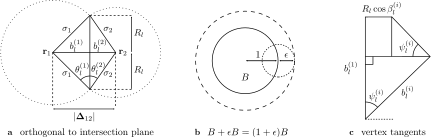
\includegraphics[width=0.9\linewidth,center]{minkowski-addition}
  \caption[Minkowski addition and difference]{
    Minkowski addition and difference.
    Note how these are not inverse operations.}
\end{SCfigure}

Distances between sets: the Hausdorff metric.

\begin{theorem}{Steiner's formula for parallel volumes}
  For a compact, convex body $K \in \mathcal{K}$ the parallel volume is expressable as:
  \begin{equation}
    \mu_d(K + \epsilon B_d) =
    \sum_{i=0}^d \mu_i(K) \omega_{d-i} \epsilon^{d-i}
  \end{equation}
\end{theorem}

\subsection{Kinematic formulae}

Motivate: usefulness in evaluating partition functions.
Probability of particles `hitting' one another.
Develop notation.

It is usual for liquid state theories to focus on spherically symmetric potentials, however integral geometry more naturally deals with non-spherical objects so we can consider this generalisation at the small cost of additional notation.
In addition to integrations over particle positions $\{\vec{r}_1, \cdots, \vec{r}_n\}$ we also have to consider their orientations $\{\vec{\theta}_1, \cdots, \vec{\theta}_n\}$ where each $\vec{\theta}_i$ represents an Euler angle tuple.
Then, assuming an isotropic phase where all orientations are equally likely each positional integral generalises to
\begin{equation*}
  \int_{\mathbb{R}^d} d\vec{r}
  \to
  \int_{\mathbb{R}^d \times SO(d)} d\vec{r} d\vec{\theta}
  :=
  \int_{G_d} dg,
\end{equation*}
with the normalisation in the angular measure such that $\int d\vec{\theta} = 1$. In the right-most equality we introduced the rigid motion operation acting on a body $A \subset \mathbb{R}^d$ as
\begin{equation*}
  g A := \{\mathcal{R}(\vec{\theta}) \vec{a} + \vec{r} \, | \, \vec{a} \in A\},
  %(\mathcal{T} \circ \mathcal{R})(\vec{r}, \vec{\theta}),
\end{equation*}
a member of the rigid motion group $g \in G_d := \mathbb{R}^d \times SO(d)$, and where $\mathcal{R} \in SO(d)$ is the rotation matrix parameterised by $\vec{\theta}$.
We can take standard results for simple liquids interacting via spherically symmetric pair potentials, and make the above replacement to obtain the correct generalisation for arbitrary shapes.

\begin{theorem}{Principal kinematic formula}
  Noting that $\chi = V_0$ is the lowest order intrinsic volume, the latter line of \eqref{eq:low-density-insertion} is ideally suited to a treatment within integral geometry.
  A central result of this field is the principal kinematic formula of Blaschke and Santal\'o \cite{BlaschkeMZ1936,Blaschke1937,SantaloASI1936} which gives the explicit form of integrals of this type as \cite{Santalo2004,Klain1997}
  %\cite{Santalo2004,SchneiderACIG1984,Schneider2008,Klain1997}
  \begin{equation}\label{eq:binomial-kinematic-formula}
    \int_{G_d} \chi(A \cap gB) \, dg
    =
    \sum_{k=0}^d (C_{k,d-k})^{-1} V_k(A) V_{d-k}(B)
  \end{equation}
  We see the flag coefficients \eqref{eq:flag-coefficients} play an analogous role in conjugating the intrinsic volumes above as binomial coefficients do in algebraic expansions%
  \marginfootnote{For this reason Klain and Rota argue that integral geometry should be called \emph{continuous combinatorics} \cite{Klain1997}, because it generalises combinatorial results to continuous spaces}.
  More general formulas exist for integrals over other intersection intrinsic volumes \cite{Klain1997}, however these do not have an interpretation in terms of evaluating partition functions so we will not use them.
\end{theorem}

The principal kinematic formula \eqref{eq:binomial-kinematic-formula} can be iterated for the intersections of many bodies $\{K_i\}$ giving \cite{Santalo2004,MarechalPRE2014}
\begin{subequations}\label{eq:multinomial-kinematic-formula}
  \begin{equation}
    \Lambda_{s_1, \cdots, s_n}
    =
      \sum_{\substack{i_0, \cdots, i_n = 0 \\ i_0 + \cdots + i_n = nd}}^d
      (C_{i_0, \cdots, i_n})^{-1}
      V_{i_0}(K_0)
      \prod_{j=1}^n
      \widetilde{V}_{i_j}(K_{s_j})
  \end{equation}
  \begin{equation}
    \textrm{with} \qquad
    C_{i_0, \cdots, i_n}
    := \frac{1}{i_0! \omega_{i_0}}
    \prod_{j=1}^n
    \left(
    \frac{d!}{i_j!} \frac{\omega_d}{\omega_{i_j}}
    \right)
  \end{equation}
\end{subequations}
where $C_{i_0, \cdots, i_n}$ would be the multinomial generalisation of the flag coefficients \eqref{eq:flag-coefficients}.
We will use this iterated formula in chapter \ref{chapter:resummation} to resum a piece of the virial series (introduced in section \ref{sec:virial-series}).

%% We have the invariant measure on 1-dimensional linear subspaces of $\mathbb{R}^d$ (\emph{Grassmanians}) as
%% \begin{equation}
%%   [d] = \tau_d(\textrm{Gr}(d,1))
%%   = \frac{d \omega_d}{2 \omega_{d-1}}.
%% \end{equation}
%% Factorial defined as
%% \begin{equation}
%%   [k]! = \prod_{i=0}^k \, [i]
%% \end{equation}
%% Flag coefficients from binomial coefficients
%% \begin{equation}
%%   {d \brack k}
%%   := \frac{[n]!}{[k]! [n-k]!}
%%   = {d \choose k}
%%   \frac{\omega_d}{\omega_k \omega_{d-k}}
%% \end{equation}
%% Provides the generalisation of combinatorial results to continuous spaces.
%% Analagously to binomial coefficients, the flag coefficients obey
%% \begin{equation}\label{eq:flag-coefficients-symmetry}
%%   {d \brack k} = {d \brack d - k}.
%% \end{equation}
%% Note that we can rewrite \eqref{eq:intrinsic-volume-ball} using the flag coefficients as
%% \begin{equation}\label{eq:intrinsic-volume-ball-flag}
%%   \mu_k (B_d) = {d \choose k} \frac{\omega_d}{\omega_{d-k}}
%%   = {d \brack k} \omega_k
%% \end{equation}

%% \begin{center}
%% \begin{tabular}{cccccc}
%%   \toprule
%%   $k$ & $\omega_k$ & $[k]$ & $[k]!$ & ${2 \brack k}$ & ${3 \brack k}$ \\
%%   \midrule
%%   0 & 1 & 1 & 1 & 1 & 1 \\
%%   1 & 2 & 1 & 1 & $\frac{\pi}{2}$ & 2 \\
%%   2 & $\pi$ & $\frac{\pi}{2}$ & $\frac{\pi}{2}$ & 1 & 2 \\
%%   3 & $\frac{4\pi}{3}$ & 2 & $\pi$ & & 1 \\
%%   \bottomrule
%% \end{tabular}
%% \end{center}

%% \begin{theorem}{General kinematic formula}
%%   For $0 \le k \le d$:
%%   \begin{equation}
%%     \int_{\mathbb{E}_d} \mu_k (A \cap g B) \, dg =
%%     \sum_{i=0}^{d-k}
%%     {i + k \brack k} {d \brack i}^{-1}
%%     \mu_{i+k}(A) \mu_{d-i}(B)
%%   \end{equation}
%%   \begin{equation*}
%%     \int_{\mathbb{E}_d} \mu_k (A \cap g B) \, dg =
%%     \sum_{i=0}^{d-k}
%%     {i + k \brack k}
%%     {d \brack i + k}
%%     \kappa_{i+k}(A) \kappa_{d-i}(B)
%%   \end{equation*}
%%   In regular binomial:
%%   \begin{equation*}
%%     \int_{\mathbb{E}_d} \mu_k (A \cap g B) \, dg =
%%     \sum_{i=0}^{d-k}
%%     {i + k \choose k} {d \choose i}^{-1}
%%     \frac{\omega_{i+k} \omega_{d-i}}{\omega_k \omega_d}
%%     \mu_{i+k}(A) \mu_{d-i}(B)
%%   \end{equation*}
%% \end{theorem}

%% \begin{equation*}
%%   {n \choose k} {k \choose p}
%%   =
%%   \frac{n!}{k!(n-k)!}
%%   \frac{k!}{p!(k-p)!}
%%   =
%%   \frac{n!}{p!(k-p)!(n-k)!}
%%   =
%%   {n \choose p, k-p, n-k}
%% \end{equation*}
%% I.e. this is a trinomial coefficient.
%% So we have
%% \begin{equation*}
%%   {n \brack k} {k \brack p}
%%   =
%%   {n \choose k}
%%   {k \choose p}
%%   \frac{\omega_n}{\omega_k \omega_{n-k}}
%%   \frac{\omega_k}{\omega_p \omega_{k-p}}
%%   =
%%   {n \choose p, k-p, n-k}
%%   \frac{\omega_n}{\omega_p \omega_{k-p} \omega_{n-k}}
%% \end{equation*}
